\documentclass[11pt]{article}
%\usepackage[utf8]{inputenc}
\usepackage{geometry,amsmath,color,graphicx,latexsym,amsfonts}
\usepackage{algorithm}
\usepackage{algpseudocode}
\usepackage{verbatim}
\usepackage{subcaption}
%\usepackage{authblk}
\geometry{margin=1in}

% %opening
\title{Finding Parallelism in the Edge-Weighted Page Rank Problem}
\author{Sam Estes, Tim Smith, Siddhant Wahal, Gopal Yalla}
\date{May 10, 2017}
%\institute{CSE 392: Parallel Algorithms \\ Final Report}

%% --- New commands
\newcommand{\pderiv}[3][]{% \pderiv[<order>]{<func>}{<var>} 
  \ensuremath{\frac{\partial^{#1} {#2}}{\partial {#3}^{#1}}}}
\newcommand{\R}{\mathbb{R}}
\newcommand{\red}[1]{\textcolor{red}{#1}}
\newcommand{\blue}[1]{\textcolor{blue}{#1}}
\newcommand{\degSym}{$^{\circ}$}
\newcommand{\noi}{\noindent}
\newcommand{\bigo}[1]{\mathcal{O}\left( #1 \right)}

% --- Parallel algorithm commands
\algblock{ParFor}{EndParFor}
\algnewcommand\algorithmicparfor{\textbf{parfor}}
\algnewcommand\algorithmicpardo{\textbf{do}}
\algnewcommand\algorithmicendparfor{\textbf{end\ parfor}}
\algrenewtext{ParFor}[1]{\algorithmicparfor\ #1\ \algorithmicpardo}
\algrenewtext{EndParFor}{\algorithmicendparfor}

%\renewcommand\Authfont{\small}
%\renewcommand\Affilfont{\itshape\footnotesize}
\begin{document}

\maketitle
\thispagestyle{empty}

\newpage
\thispagestyle{empty}
\tableofcontents
\newpage
\setcounter{page}{1}

%%%%%%%%%%%%%%%%%%%%%%%%%%%%%%%%%%%%%%%%%%%%%%%%%%%%%%%%%%%%
%% 1. Introduction
%%%%%%%%%%%%%%%%%%%%%%%%%%%%%%%%%%%%%%%%%%%%%%%%%%%%%%%%%%%%

\section{Introduction}

We consider the problem of ranking webpages on the internet based on a user's
query. We view the internet as a graph where the webpages are nodes and the
links are edges. 
In the PageRank problem a random walker moves across a graph, transitioning to
adjacent nodes along an edge or jumping to a new, non-adjacent node. The
distribution of positions for a walker at time $t$ is given by the discrete-time
Markov process: 

\begin{equation}
        x^{(t+1)}=\alpha P x^{(t)} + (1-\alpha) v \; ,
\label{eq:pagerank_markov}
\end{equation}

\noi where $P$ is the edge transition probability matrix and $v$ represents jump or
teleport probabilities. Here $\alpha$ is the edge
transition probability (i.e. how likely the walker is to transition to an
adjacent node), and $(1-\alpha)$ represents the teleport probability (e.g. the
probability a user goes to a webpage in their bookmarks rather clicking a link).
Defining $w$ as a vector of personalization parameters specified by the user's
query, we seek to solve the
edge-weighted personalized PageRank problem: 

\begin{equation}
        Mx=b
\label{eq:pagerank_linear}
\end{equation}

\noi where $M(w) = (I-\alpha P(w))$ and $b = (1-\alpha)v(w)$, and $w \in
\mathbb{R}^d$ is
the \textit{personalization vector}, which specifies the topic preference for
a given query. 

In general, computing the edge-weighted personalized page rank vector is expensive
and not feasible for online, interactive situations. \cite{xie} present a
solution to this problem, where they solve Eqn. (\ref{eq:pagerank_linear}) for many
sample queries preemptively (i.e. in an ``offline'' computation). They find low
dimensional subspaces for
approximating each of these samples and solve a constrained least squares
problem to estimate the PageRank vector in an ``online'' query. The solution to
these low dimensional systems can be computed almost immediately, such that
a user can query a database at interactive speeds.   

Since the algorithm presented in \cite{xie} already achieved interactive speeds, it seemed
unnecessary to try to formulate a parallel implementation. Therefore we looked
to improving the more expensive offline computation, which solves Eqn.
(\ref{eq:pagerank_linear}) exactly. Speeding up this computation could allow for
an implementation presented by \cite{xie} where the database is updated
frequently, requiring successive offline computations for producing sample
PageRank vectors.

The sequential complexity for solving Eqn. (\ref{eq:pagerank_linear}) amounts to
solving iteratively applying a MatVec (e.g. for a Jacobi iteration), which is
naively $\mathcal{O}(N^2)$ complexity. In our approach, we first reorder the
matrix $M$ by successively coarsening the related adjacency matrix and
implementing a spectral bisection algorithm to improve data locality. We then
solve Eqn. (\ref{eq:pagerank_linear}) with a Jacobi iterative scheme motivated
by the Markov process given by Eqn. (\ref{eq:pagerank_markov}). Here all
matrices and vectors are stored using Compressed Sparse Column (CSC) format. We
implemented our method using a shared memory approach in C++ using OpenMP on the Knights Landing (KNL) processors on
Stampede. We tested our methods on the DBLP computer science citation database
\cite{dblp} and a network of facebook users \cite{facebook}, where these
datasets were found from the SNAP website \cite{snapnets}. 

We found that the computations involved with reordering the matrix $M$ (i.e.
coarsening and spectral bisection) were much more complex than simply solving
the linear system. The key here was rewriting the linear solver to handle the
CSC format, and only perform computations for nonzero entries of the right hand
side, $b$. Thus while the coarsening and reordering strategies are theoretically
very interesting and scaled well up to 32 cores on the KNL nodes, 
we did not find them useful for this particular application. 


%%%%%%%%%%%%%%%%%%%%%%%%%%%%%%%%%%%%%%%%%%%%%%%%%%%%%%%%%%%%
%% 2. Methodology
%%%%%%%%%%%%%%%%%%%%%%%%%%%%%%%%%%%%%%%%%%%%%%%%%%%%%%%%%%%%

\section{Methodology}

Our problem takes the view of a network of users in the facebook data or
citations in the DBLP database. Two vertices are connected by an edge when e.g. two
users are friends on facebook or when one paper cites another in the DBLP graph.
These graphs are highly sparse, and randomly ordered.
The algorithm we implemented follows three basic steps: (1) successively coarsen
the graph to reduce the number of effective nodes, (2) reorder the graph via
spectral bisection, and (3) solve the linear system with a Jacobi iterative
method motivated by Eqn. (\ref{eq:pagerank_markov}) in Compressed Sparse
Column (CSC) format. We discuss each of these separate parts in detail here. 

\subsection{Graph Coarsening}

The graph coarsening algorithm involves two intermediate phases. First, we
labeled each node in the graph with a color by repetitively computing Maximal
Independent Sets (MIS), where each color makes a maximal independent set for the
graph. The pseudocode for the MIS algorithm is shown in
Algorithm \ref{alg:mis}. The coloring algorithm is neglected for brevity since
it merely involves iteratively computing the MIS of a graph, assigning a
different color each time. Next, we used the
graph colors to match the nodes into pairs in a maximal matching algorithm. Here
it was important to assign partners such that the edgeweight between them is
maximized in order to minimize the edges between the two groups of nodes formed
by the spectral bisection algorithm. The pseudocode for maximal matching is
shown in Algorithm \ref{alg:mxm}. 

%%% MIS Algorithm
	\begin{algorithm}[H]
        \small
	\caption{Maximal Independent Sets}\label{alg:mis}
	\begin{algorithmic}[1]
	\Procedure{mis\_shared}{Graph g, vector colored, vector I}
        \State{\textit{g: graph containing node and edge information}}
        \State{\textit{colored: vector of nodes already assigned a color}}
        \State{\textit{I: vector to fill of independent nodes}} \\

        \State{$C=g.nodeList\,\, s.t.\,\, (g.nodeList\cap colored==\emptyset)$} 
	\ParFor{$i=0:C.size$}
        \State{$r[i] = rand(0,(C.size)^4)$}
        \EndParFor

        \While{$!isEmpty(C)$}
        \State{$removeFlag[i\in C]=false$}
        \State{$keepFlag[i\in C]=false$}

        \ParFor{$i \in C$}
        \For{$j \in g.neighborsOf[i]$}
        \If{$r[i]>r[j]$}
        \State{keepFlag[i]=true}
        \Else
        \State{removeFlag[i]=true}
        \EndIf
        \EndFor
        \EndParFor

        \ParFor{$i \in C$}
        \If{$ (!(keepFlag[i])\, \&\&\, (removeFlag[i])) \,||\, isEmpty(g.neighborsOf[i])$}
        \State{C.pop(i)}
        \State{I.push(i)}
        \EndIf
        \EndParFor

        \ParFor{$u\in I$}
        \For{$j \in g.neighborsOf[u]$}
        \State{C.pop(j)}
        \EndFor
        \EndParFor

        \EndWhile

	\State{\textbf{return} I }
	\EndProcedure
	\end{algorithmic}
	\end{algorithm}

%%% MXM algorithm        

	\begin{algorithm}[H]
        \small
	\caption{Maximal Matching}\label{alg:mxm}
	\begin{algorithmic}[1]
	\Procedure{mxm\_shared}{Graph g, vector colors, vector matchList}
        \State{\textit{g: graph containing node and edge information}}
        \State{\textit{colors: vector of colors for each node}}
        \State{\textit{matchList: vector containing node pairs}}\\
        \For{$k=0:max(colors)-1$}
        \State{nodeList = parallel\_select\_shared(unmatched nodes, color==k)}
        
        \ParFor{$u \in nodeList$}
        \State{v = find\_unmatched\_max\_edgeweight(g.neighborsOf[u])}
        \State{matchList[u] = v; matchList[v]=u}
        \State{raceList.push(u)}
        \EndParFor

        \ParFor{$u \in raceList$}
        \If{$matchList[matchList[u]] \,!=\, raceList[u]$}
        \State{matchList[u] = unmatched}
        \EndIf
        \EndParFor

        \EndFor
        
        \State{\textbf{return} matchList}
        \EndProcedure
        \end{algorithmic}
        \end{algorithm} 


\subsection{Spectral Bisection}
The goal of spectral bisection is to reorder a matrix in such a way that the number of off diagonal non-zero
elements is reduced; this can lower the overhead (e.g., communication) during a parallel
matrix-vector multiplication. To perform a spectral bisection, one must form the
graph laplacian, compute the eigenvector cooresponding to the least significant
eigenvalue, and then reorder the graph according to median value of the
eigenvector. Performing a spectral bisection is expensive due to the eigenvalue
computation and is not feasible on most data sets. This generates the need for
the coarsening methods discusses earlier. 


\subsection{Iterative Linear Solver}

As discussed in the first section, we use a Jacobi method to solve Eqn.
(\ref{eq:pagerank_linear}). The iterative solver is defined by the recusive
algorithm:

\begin{equation*}
	x_{n+1} = \alpha AD^{-1}x_{n}+(1-\alpha)v \; , 
\end{equation*}

\noi where $A$ is the adjacency matrix of the graph and $D$ is the diagonal
matrix of node degrees. The above computation is consumed by the matrix-vector
multiplication. We make use of CSC format to perform the matvec. This
significantly reduces the storage cost as well as the required number of
computations. A CSC matrix is defined by three vectors, \textit{vals,irow,} and
\textit{pcol}. \textit{Vals} stores the values of the non-zero elements of the
given matrix; \textit{irow} stoes the row index of the non-zero elements of the
given matrix, and \textit{pcol} stores pointers to the element that start each
new column. It's important to note that \textit{pcol} is defined with the
following relationship in order to deal with all zero columns: 

\begin{equation*}
	\begin{split}
		\rm{pcol}[0] &= 0\\
		\rm{pcol}[i] &=
		(NNZ\;in\;column\;i-1)
		+ \rm{pcol}[i-1]
	\end{split}
\end{equation*}

The algorithm for a CSC matvec where $x$ is assumed to also be
sparse and stored in CSC format is given in algorithm \ref{CSC}.

\begin{algorithm}[H]
\caption{CSC Matrix-CSC Vector Multiplication}\label{CSC}
\begin{algorithmic}[1]
\Procedure{CSC\_MatVec}{CSC A,CSC x}
\State{Set $b$ to zero}
\ParFor{$j=0:x.irow.size()-1$}
\For{$i=A.pcol[x.irow[j]]:A.pcol[x.irow[j]+1]-1$}
\State{$b[A.irow[i]] += A.vals[i]*x.vals[j]$}
\EndFor
\EndParFor
\State{\textbf{return} b }
\EndProcedure
\end{algorithmic}
\end{algorithm}

%%%%%%%%%%%%%%%%%%%%%%%%%%%%%%%%%%%%%%%%%%%%%%%%%%%%%%%%%%%%
%% 3. Experimental setup
%%%%%%%%%%%%%%%%%%%%%%%%%%%%%%%%%%%%%%%%%%%%%%%%%%%%%%%%%%%%
\section{Experimental Setup}
\subsection{Implementation Details}

In order to test our methodology, we wrote a C++
package called {\rm SPARC} (Sparse PAge Rank in C). Given a
graph, our pacakge can solve the page rank problem using a combination of coarsening, spectral
bisection, and a parallel matvec with CSC formatted data inside a Jacobi
iterator. The code was built on the ICES machines, as well as on \textit{Stampede 2} at TACC using the gnu
compilers g++/gcc. Regarding external dependencies, {\rm SPAC}, makes use of
{\rm ARPACK}, {\rm SuperLU}, and {\rm Boost}. {\rm ARPACK} is used in conjuction
with {\rm SuperLU} to solve for the two least significant eigenvalues and
eigenvectors of a given
matrix; this is the same package used by the Matlab function ``eigs()''. {\rm
Boost} program options is used for the API. Our package comes with two
makefiles: one for KNL, which requires the use of Intel's MKL package for BLAS
and LAPACK, and one for the ICES desktops and similar machines. Issuing a `make
dep' will build all external dependencies. Moreover, issuing a `make install' will
build the source code and issuing a `make check' command will run the unit test suite.  

\subsection{List of Experiments}

Aside from the test suite in the code, which contains small example graphs
for verification purposes, we tested our code on two main datasets: The DBLP
collaboration network dataset and the Facebook social circles data set
\cite{snapnets,facebook,dblp}. For the Facebook data, our goals we as follows: 

\begin{itemize}
	\item Test the correctness of spectral bisection with the example given in
		class. 
		\begin{itemize}
			\item Expected the results to match and they did.
		\end{itemize}
	\item See how different coarsening levels affect the results of spectral bisection,
		i.e., the number of non-zeros in the off diagonal. 
		\begin{itemize}
			\item Expected to see not much of a different. 
			\item Observed that the coarsening/uncoarsening process can
				severly dampen the effective reordering of
				spectral bisection.
		\end{itemize}
	\item Understand the tradeoff between spectral bisection time and
		coarening levels. 
		\begin{itemize}
			\item Expected spectral bisection to take a long time,
				and for coarsening to be cheap and thus lead to
				a faster but similar spectral bisection. 
			\item Observed that while coarsening is faster than
				spectral bisection, the act of coloring is still
				to slow for practicle purposes.
		\end{itemize}
\end{itemize}
\noi Similarly, for the DBLP data set, our goals were to: 

\begin{itemize}
	\item See how much of a difference spectral bisection makes when solving
		a sparse matvec on shared memory (and different memory
		configurations on Stampede 2). 
		\begin{itemize}
			\item Expected spectral bisection to greatly speed up
				calculation. 
			\item Observed negligible speed up.
		\end{itemize}
	
	\item Determine strong scaling results of coarsening on Stampede 2. 
		\begin{itemize}
			\item Observed linear scaling. 
		\end{itemize}
	\item Determine the speedup involved by performing a CSC matvec within a
		jacobi iterator. 
		\begin{itemize}
			\item Expected the majority of the speed up to come from
				the spectral bisection process. 
			\item Observed that the true speed up came from using a
				CSC format, so that all the data could fit
				easily in main memory. 
		\end{itemize}
	\item Compare the times with the results from \cite{xie}.
		\begin{itemize}
			\item In the end we sped up their offline calculations
				from 6 hours to 25 minutes, by using a sparse
				matvec with CSC format. 
		\end{itemize}
\end{itemize}

%%%%%%%%%%%%%%%%%%%%%%%%%%%%%%%%%%%%%%%%%%%%%%%%%%%%%%%%%%%%
%% 4. Results
%%%%%%%%%%%%%%%%%%%%%%%%%%%%%%%%%%%%%%%%%%%%%%%%%%%%%%%%%%%%
\section{Results}
\subsection{Facebook Data}

\begin{figure}
\centering
\begin{subfigure}{.5\textwidth}
	\centering
	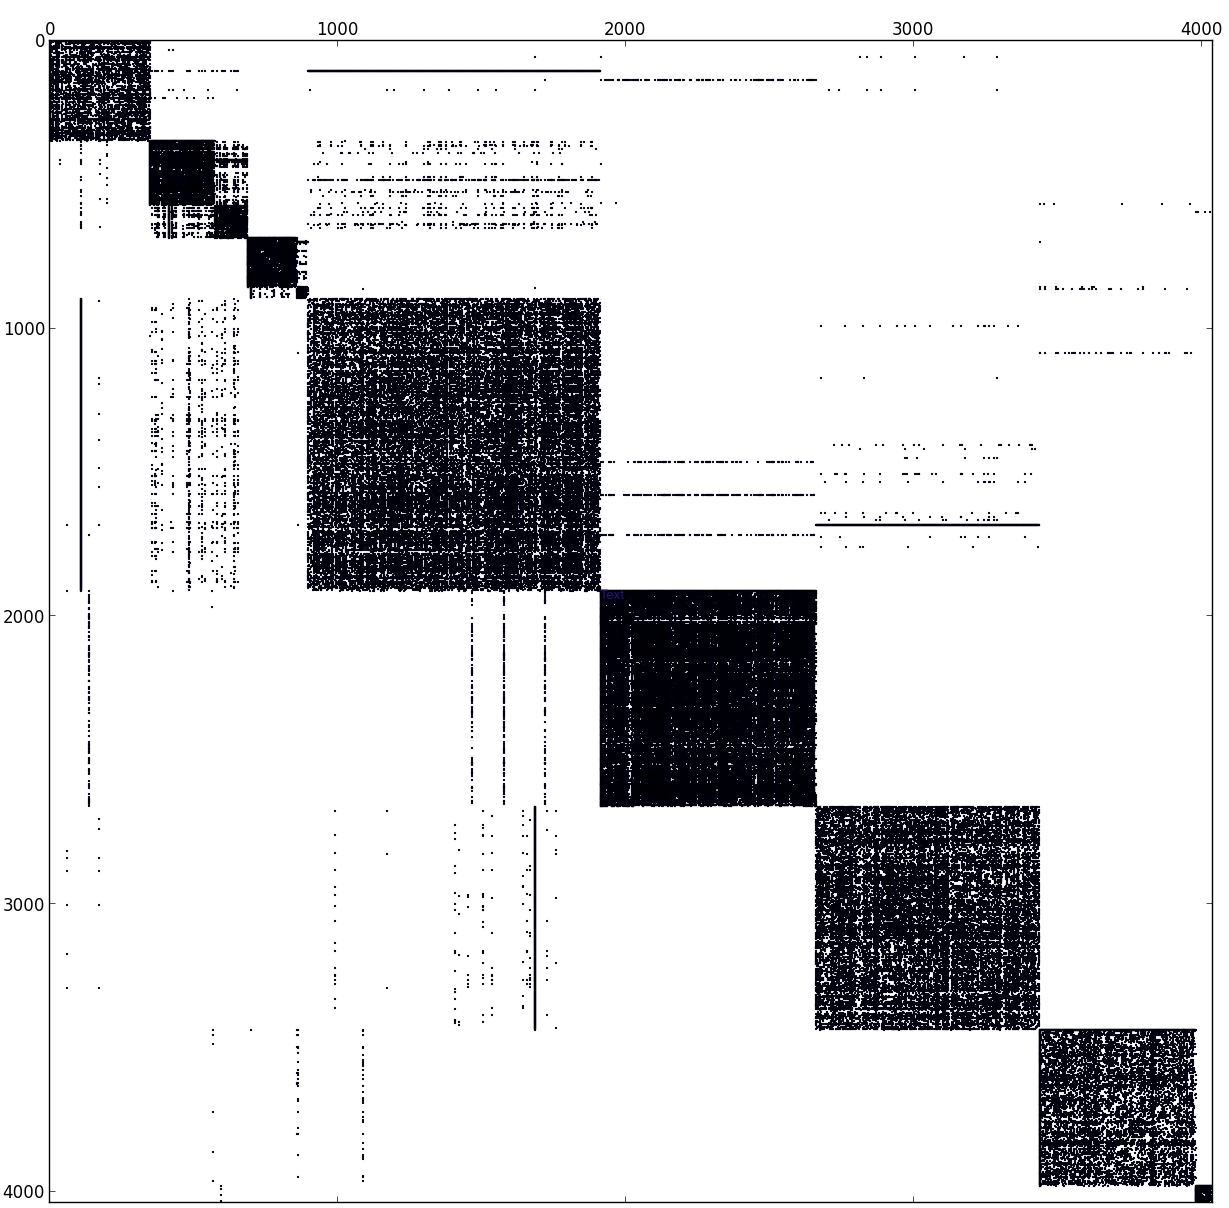
\includegraphics[width=.9\linewidth]{figs/Facebook_Original.png}
	\caption{Original Facebook Data}
	\label{fig:FB}
\end{subfigure}%
\begin{subfigure}{.5\textwidth}
		\centering
		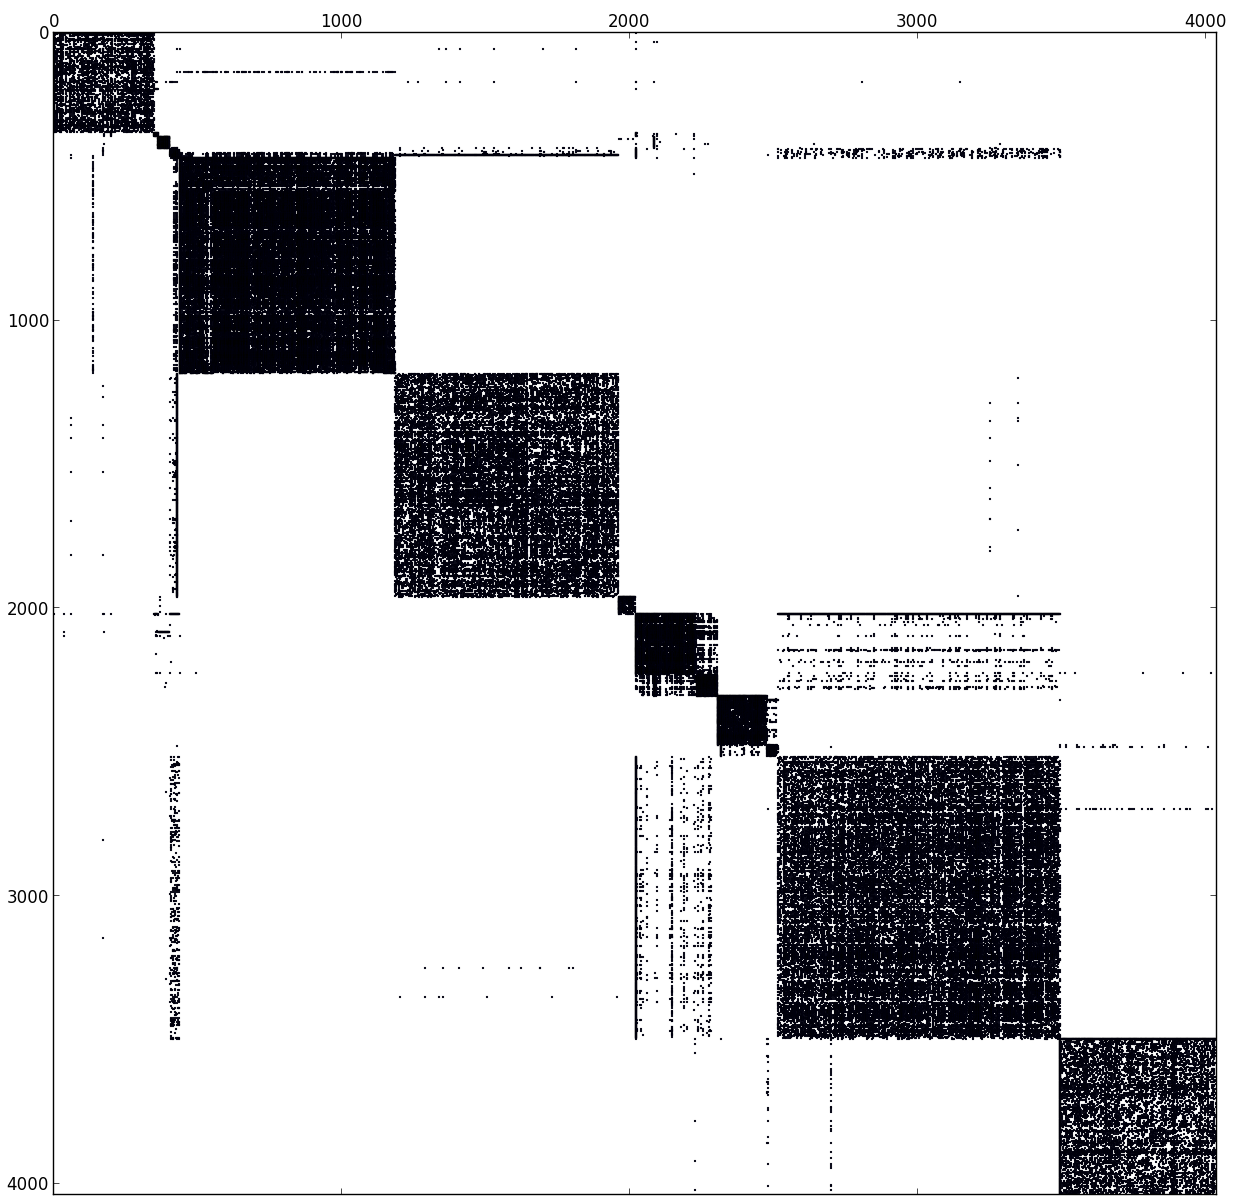
\includegraphics[width=.9\linewidth]{figs/Facebook_SB_C0.png}
		\caption{Facebook Data after Spectral Bisection}
		\label{fig:sub2}
	\end{subfigure}
	\caption{ (a) The original facebook data. Total number of
non-zeros is 88234 and and number of off diagonal non-zeros is 16466. (b)
Facebook data after spectral bisection. The number of off diagonal blocks
reduced to 1266. } 
	\label{fig:FBSB}
\end{figure}
\begin{figure}
\centering
\begin{subfigure}{.5\textwidth}
	\centering
	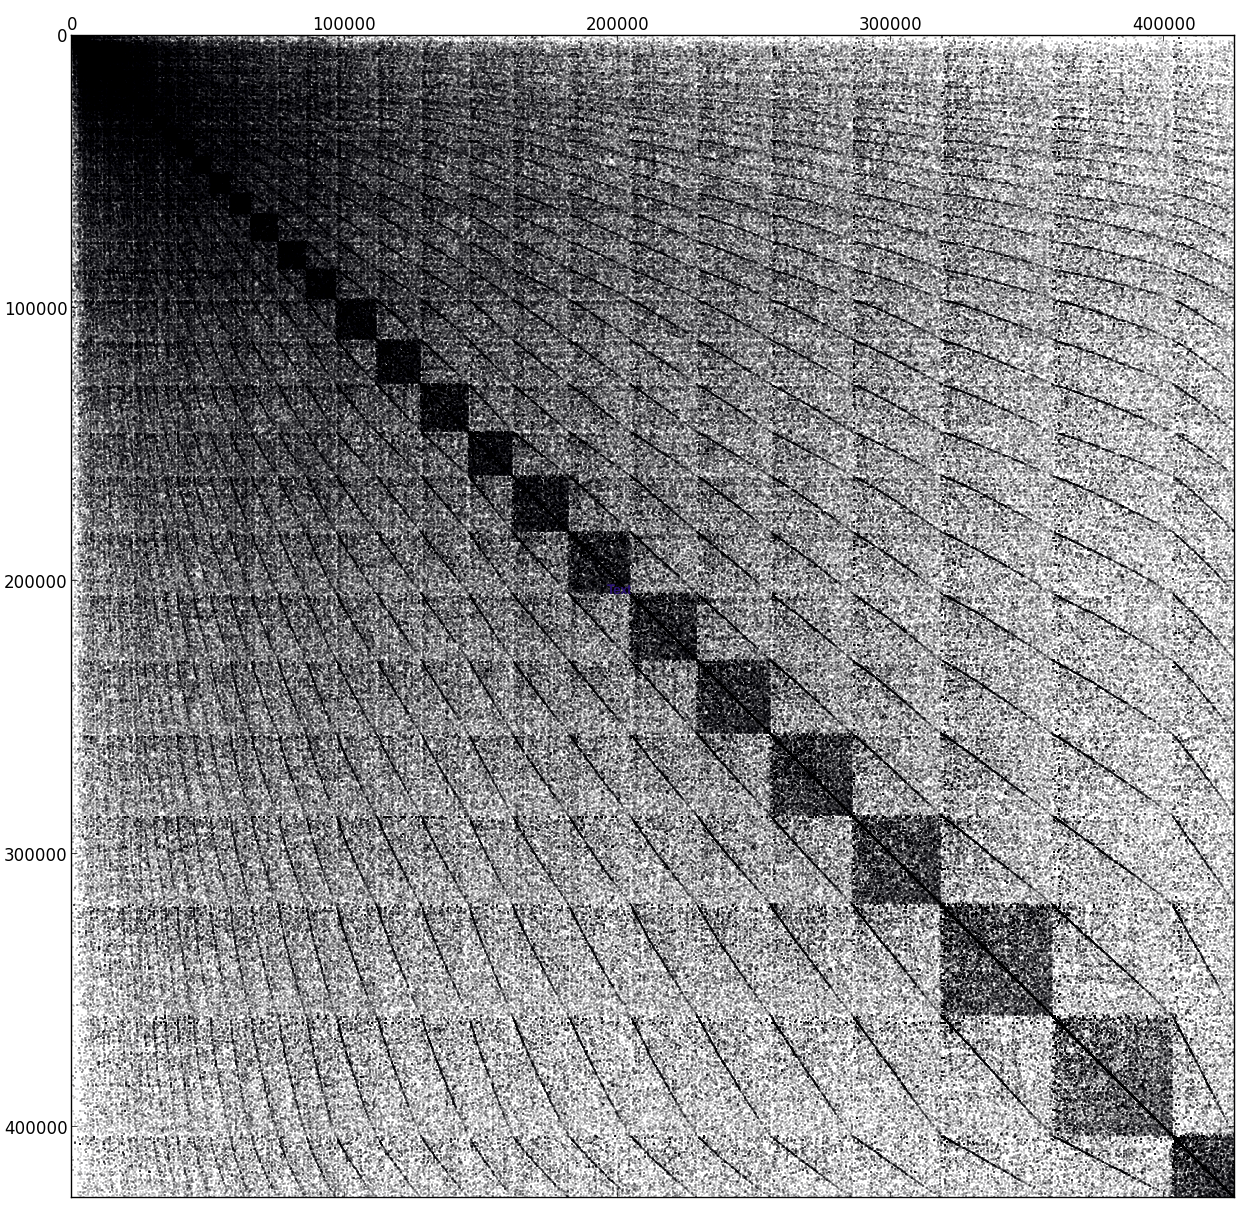
\includegraphics[width=.9\linewidth]{figs/DBLP_Original.png}
	\caption{DBLP Original Data}
	\label{fig:DBLP_SB_C0}
\end{subfigure}%
\begin{subfigure}{.5\textwidth}
		\centering
		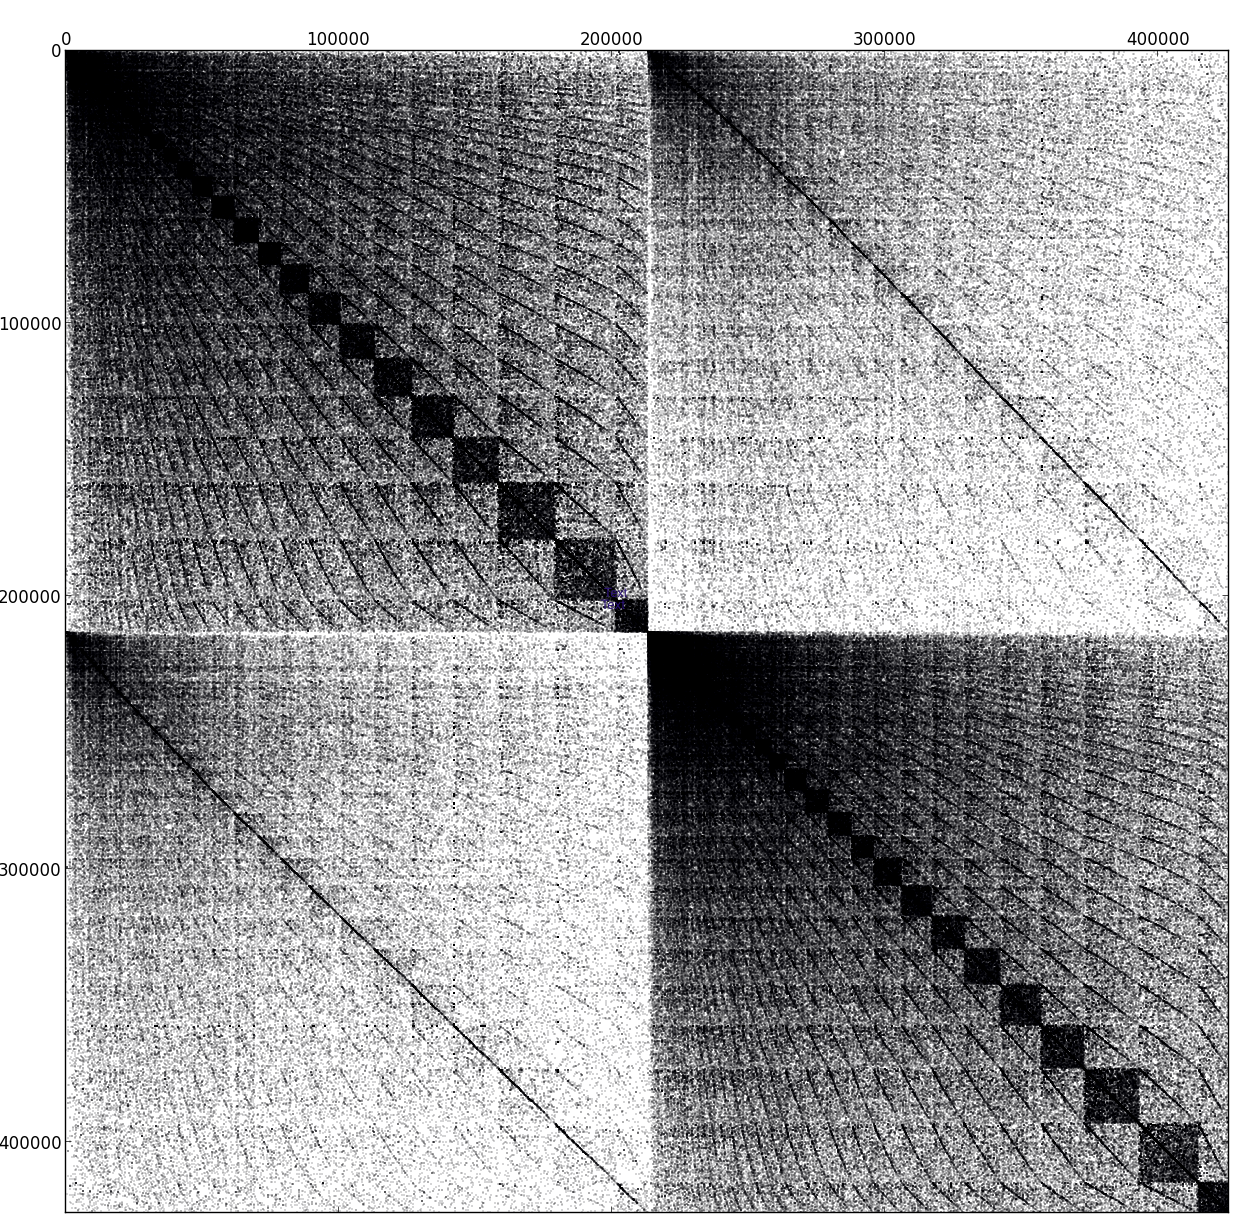
\includegraphics[width=.9\linewidth]{figs/DBLP_SBC0.png}
		\caption{DBLP after Spectral Bisection}
		\label{fig:DBLP_SB_C4}
	\end{subfigure}
	\caption{ (a) The original DBLP data. Total number of
non-zeros is 1049866 and and number of off diagonal non-zeros is 628800. (b)
DBLP data after spectral bisection. The number of off diagonal blocks
reduced to 350038. } 
	\label{fig:DBLPSB}
\end{figure}

\begin{figure}
	\centering
	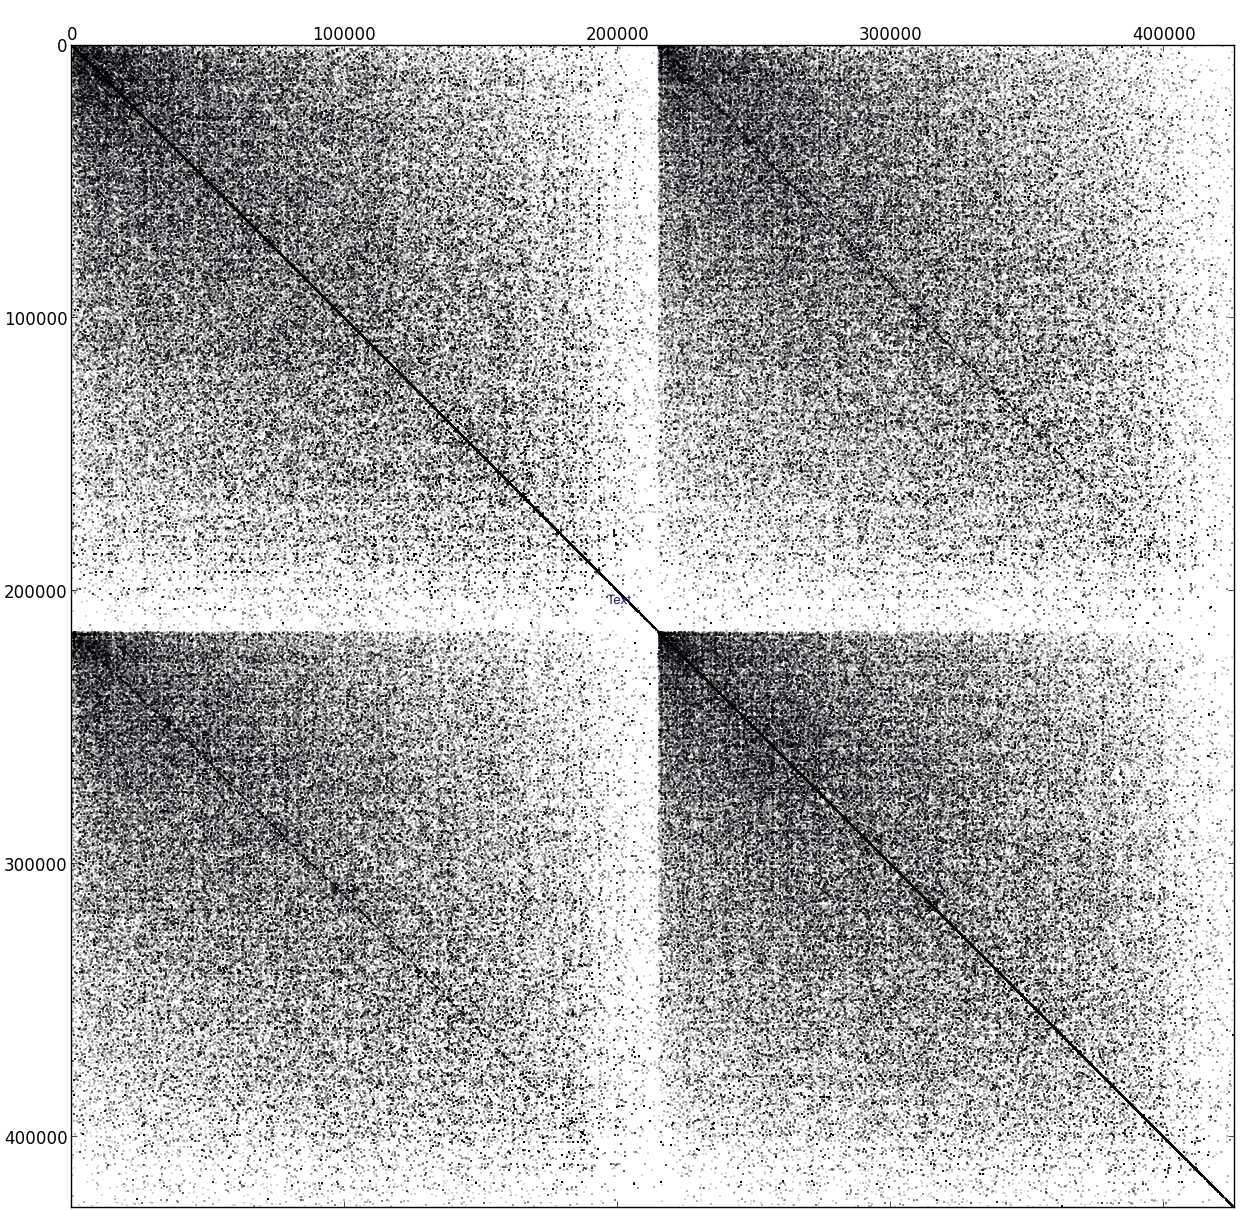
\includegraphics[width=0.5\linewidth]{figs/DBLP_SBC4.png}
	\caption{DBLP data after four coarsens and then spectral bisection. The
	number of off diagonals reduced slightly to 523194.}
	\label{fig:DBLP}
\end{figure}



%%%%%%%%%%%%%%%%%%%%%%%%%%%%%%%%%%%%%%%%%%%%%%%%%%%%%%
% CITATIONS
%%%%%%%%%%%%%%%%%%%%%%%%%%%%%%%%%%%%%%%%%%%%%%%%%%%%%%%%%%%
\newpage

%\addcontentsline{toc}{subsubsection}{\protect\numberline{\thesubsubsection}
%  line added to TOC: subsubsection one}

\addcontentsline{toc}{section}{References} 

\bibliographystyle{ieeetr} 
\bibliography{spicy}



\end{document}

